\chapter{الدارات القصيرة والسلامة الكهربائية}\label{ch:g7:short-circuits-safety}

كل قاعدة سلامة تعلّمتها ترجع إلى شرّير واحد لقيته لمحةً في
السنة الماضية: \omterm{def:g6:circuits-and-safety:short}{الدارة القصيرة}. وهذا الفصل يدرسه على أصوله ---
كيف يبدأ، ولماذا يحرق، وكيف يهزمه سلك متواضع يضحّي بنفسه ---
ويحوّل علبة مصاهر الأسرة من خزانة غامضة إلى حليف تفهمه.

\section{طريقة الشرّير}

\begin{proposition}[التيار يفضّل الطريق بلا جهد]\label{prop:g7:short-circuits-safety:effortless}
بين طريقين يصلان النقطتين نفسيهما، يتزاحم التيار السائر على
الطريق الذي يقاومه أقلّ. والعناصر --- المصابيح والمحرّكات
والطنّانات --- كلها تقاوم المسير وهي تعمل؛ أما سلك غليظ بسيط
فلا يكاد يقاومه. فاعرِض على المسير التفافًا بسلك عارٍ يهجر
الطريق العامل هجرًا شبه تامّ إلى الطريق بلا جهد.
\end{proposition}

\begin{definition}[الدارة القصيرة على عنصر]\label{def:g7:short-circuits-safety:device}
يكون العنصر \emph{مقصورًا}\index{دارة قصيرة} حين يصل طريق \omterm{def:g4:conductors-insulators:conductor}{ناقل}
طرفيه مباشرة، فيلتفّ عليه. فيهجر المسير العنصر --- فيعتم \omterm{def:g3:first-electric-circuit:bulb}{مصباح}
مقصور، ويقف محرّك --- بينما تواصل بقية الحلقة عملها، وقد صار
فيها عامل أقلّ يقاوم المسير.
\end{definition}

\begin{definition}[الدارة القصيرة على البطارية]\label{def:g7:short-circuits-safety:battery}
والحالة الأخطر: طريق \omterm{def:g4:conductors-insulators:conductor}{ناقل} يصل قطبَي \emph{\omterm{def:g3:first-electric-circuit:battery}{البطارية}} ولا عنصر
عليه البتة. فلا شيء يقاوم المسير أصلًا، فيصير اندفاعًا جامحًا
--- والاندفاع الجامح يُسخّن السلك \omterm{def:g3:first-electric-circuit:battery}{والبطارية} نفسها، فيُتلف
الخلايا، ويصهر العزل، ويُشعل البيوت على شبكة الكهرباء.
\end{definition}

\begin{method}[الشرّير، معروضًا بأمان]\label{met:g7:short-circuits-safety:demo}
\omterm{def:g3:first-electric-circuit:battery}{ببطارية} واحدة ومصباحين \omterm{def:g4:series-circuits:series}{على التسلسل} (وهو آمن: فدفع \omterm{def:g3:first-electric-circuit:battery}{البطارية}
ضئيل):
\begin{enumerate}
  \item أضِئ المصباحين --- خافتين بالتساوي، كما يعد قانون
        التسلسل؛
  \item والآن المِس بسلك بسيط طرفَي \omterm{def:g3:first-electric-circuit:bulb}{المصباح} 2، ملتفًّا عليه؛
  \item وراقب: يموت \omterm{def:g3:first-electric-circuit:bulb}{المصباح} 2 في الحال --- مهجورًا --- بينما
        يقفز \omterm{def:g3:first-electric-circuit:bulb}{المصباح} 1 \emph{أسطع}: فبالتفاف على مقاوم واحد
        يقوى مسير الحلقة كلها؛
  \item وانزع السلك: فيعود المسير إلى \omterm{def:g3:first-electric-circuit:bulb}{المصباح} 2، ويعود الخفوت
        المتساوي.
\end{enumerate}
تجربة واحدة وثلاثة دروس: قاعدة الالتفاف، والعنصر المهجور،
والاندفاع المتقوّي.
\end{method}

\begin{omfigure}
\begin{tikzpicture}[scale=0.9]
  \draw (0,0) to[battery1, l=بطارية] (0,2.8)
    to[short] (1.8,2.8)
    to[lamp, l=المصباح 1: أسطع!] (4.4,2.8)
    to[lamp, l=المصباح 2: معتم] (7.0,2.8)
    to[short] (8.4,2.8)
    to[short] (8.4,0)
    to[short] (0,0);
  \draw[very thick, omThm] (4.7,2.8) to[bend left=48] (6.7,2.8);
  \node[above, font=\small, omThm] at (5.7,3.75)
    {الالتفاف: المسير يهجر المصباح 2};
\end{tikzpicture}

{\small قصر عنصر: سلك عارٍ عبر \omterm{def:g3:first-electric-circuit:bulb}{المصباح} 2 يسرق مسيره كله ---
فيموت \omterm{def:g3:first-electric-circuit:bulb}{المصباح} 2، ويشتعل \omterm{def:g3:first-electric-circuit:bulb}{المصباح} 1، وحده في مواجهة \omterm{def:g3:first-electric-circuit:battery}{البطارية}،
أسطع.}
\end{omfigure}

\begin{example}[لماذا تسخن الأسلاك]\label{ex:g7:short-circuits-safety:heating}
التيار السائر يُدفئ طريقه قليلًا دائمًا --- وتوهّج \omterm{def:g3:first-electric-circuit:bulb}{المصباح} هو
تلك التدفئة، مسخَّرةً عن قصد في خيط مبنيّ ليعمل أبيض ساخنًا. أما
في الاندفاع الجامح فتصير التدفئة تهديدًا: إذ يستطيع اندفاع
\omterm{def:g6:circuits-and-safety:short}{الدارة القصيرة} أن يُسخّن سلكًا نحاسيًّا فوق \omterm{def:g4:changes-of-state:melting-point}{درجة انصهار} غلافه
البلاستيكي في ثوانٍ. والعرض المسبق \omterm{def:g6:mass-and-volume:volume}{بحجم} الجيب: \omterm{def:g3:first-electric-circuit:battery}{بطارية} مقصورة
بسلك تسخن في يدك --- وهي الفيزياء نفسها التي تفحّم الجدران
بمقياس الشبكة. (وأما كيف تنمو التدفئة مع الاندفاع فيُقاس على
أصوله بعد سنتين، مع فصل الاستطاعة الكهربائية.)
\end{example}

\begin{omfigure}
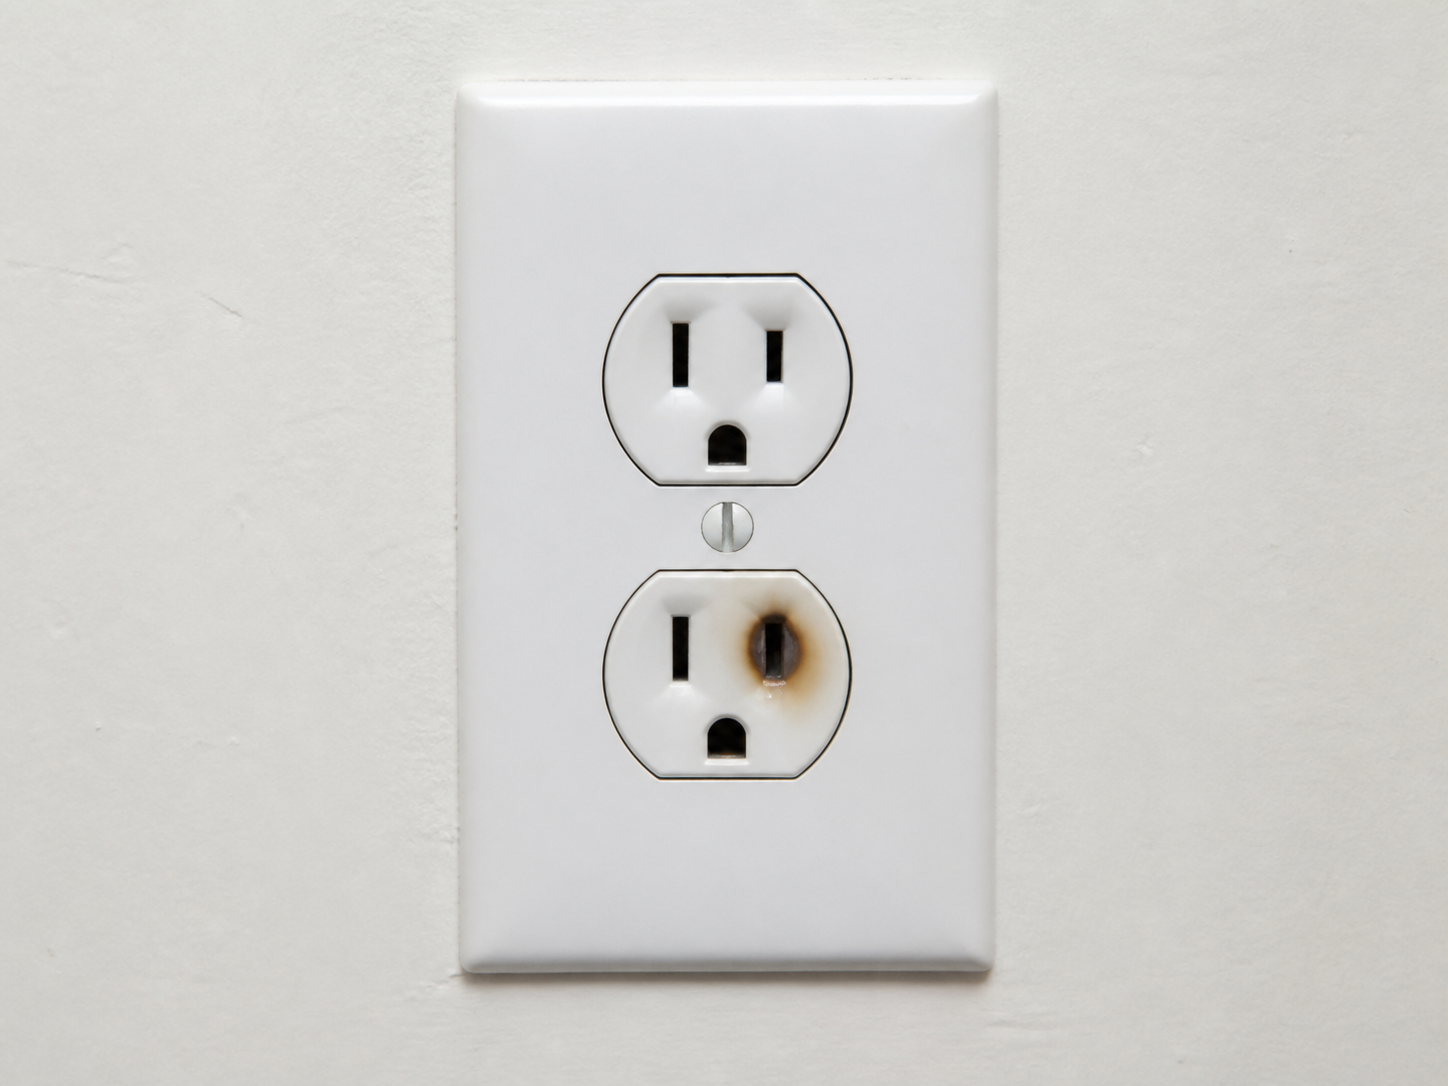
\includegraphics[width=0.45\linewidth]{images/book1/ai/g7-short-circuit-scorched.png}

{\small ما يخلّفه العطل وراءه: تيار مفرط السخونة تفحّم هذا المأخذ. وهذا هو الخطر الذي وُجد \omterm{def:g7:short-circuits-safety:fuse}{المصهر} والقاطع لإيقافه.}
\end{omfigure}

\section{الحرّاس}

\begin{definition}[المصهر]\label{def:g7:short-circuits-safety:fuse}
\emph{المصهر}\index{مصهر} حارس يموت من أجلك: سلك رفيع عن قصد،
\omterm{def:g4:series-circuits:series}{على التسلسل} مع الدارة التي يحرسها، مختار \omterm{def:g2:ice-water-steam:meltfreeze}{لينصهر} --- فيقطع
الحلقة --- حين يتجاوز التيار حدّه المقنّن. فالاندفاع الجامح
الذي كان سيفحّم أمتارًا من أسلاك البيت يُتلف بدلًا من ذلك ثلاثة
سنتيمترات من سلك مضحٍّ في خرطوشته المقاومة للنار. والمصهر
المحترق يُستبدَل --- \emph{بعد} إيجاد العطل --- بآخر جديد من
التقنين نفسه.
\end{definition}

\begin{example}[القاطع والمصهر: حارسان وواجب واحد]\label{ex:g7:short-circuits-safety:breaker}
يؤدّي قاطع الدارة الحديث واجب \omterm{def:g7:short-circuits-safety:fuse}{المصهر} من غير أن يموت: فهو قاطعة
بنابض تنفتح فجأة عند الاندفاع وتُعاد بحركة --- بعد شفاء العطل.
ومصهرًا كان أم قاطعًا، فموقع الحارس واحد: \emph{\omterm{def:g4:series-circuits:series}{على التسلسل}}،
على \omterm{def:g5:series-parallel-circuits:parallel}{الفرع} الذي يحميه، حتى يضطرّ الاندفاع إلى المرور بنقطة
تفتيشه. أما حارس \omterm{def:g5:series-parallel-circuits:parallel}{على التفرع} فيشاهد الاندفاع يهدر على الطريق
الآخر --- زينة خالصة.
\end{example}

\begin{example}[الحمل الزائد: الاندفاع المؤدَّب]\label{ex:g7:short-circuits-safety:overload}
ليس كل اندفاع خطِر دارةً قصيرة. فمشترك مآخذ يغذّي مدفأة
وغلّاية ومحمصة دفعة واحدة يطلب من فرعه الواحد أن يحمل ثلاثة
مسايير كاملة معًا --- وكل جهاز بريء، ومجموعها حمل زائد يُدفئ
أسلاك الجدار كأنها محمصة بطيئة. فيقفز القاطع على المجموع، وهو
محقّ. وقاعدة البيت: جهاز مسخِّن نهم واحد لكل مأخذ؛ ومشترك
المآخذ للمصابيح والشواحن، لا لمطبخ خاصّ.
\end{example}

\begin{remark}[الإصلاح المحرَّم]\label{rem:g7:short-circuits-safety:nail}
الحكاية القديمة صحيحة وما زالت تقتل: يظلّ \omterm{def:g7:short-circuits-safety:fuse}{مصهر} بيت يحترق،
فيصلحه أحدهم بمسمار أو بقطعة نقود --- وهو \omterm{def:g4:conductors-insulators:conductor}{ناقل} متين لن \omterm{def:g2:ice-water-steam:meltfreeze}{ينصهر}
أبدًا. فيُسكَت العَرَض؛ ويستمرّ الداء مستعرًا. ولا يلقى
الاندفاع التالي نقطة تفتيش، فتصير أسلاك البيت نفسها هي \omterm{def:g7:short-circuits-safety:fuse}{المصهر}
--- داخل الجدران. فلا تلتفّ على حارس أبدًا: \omterm{def:g7:short-circuits-safety:fuse}{فالمصهر} الذي يظلّ
يحترق حارس يظلّ يقول الصدق.
\end{remark}

\begin{remark}[القواعد في صورتها النهائية]\label{rem:g7:short-circuits-safety:rules}
كتاب قوانين الأسرة الكهربائي، وأسبابه كاملة الآن: لا تجسر
قطبَي \omterm{def:g3:first-electric-circuit:battery}{بطارية} أبدًا، وأبعِد المفاتيح المعدنية عن بطاريات
السيارات (فقصر \omterm{def:g3:first-electric-circuit:battery}{بطارية} بمعدن قوس لحام)؛ وجهاز واحد نهم \omterm{def:g5:heat-and-insulation:heat}{للحرارة}
لكل مأخذ (الحمل الزائد)؛ والأسلاك المتضرّرة تُقاعَد (فالغلاف
المتهرّئ \omterm{def:g7:short-circuits-safety:device}{دارة قصيرة} تتمرّن)؛ والماء والشبكة متباعدان، والأيدي
جافّة دائمًا (فلا يجوز أن يكون جسمك هو الالتفاف)؛ والحرّاس
محترَمون --- مصاهر مطابقة لا غير، والأعطال تُوجد قبل الإعادة؛
والمأخذ نفسه، إلى الأبد، ليس للأصابع ولا للتجارب.
\end{remark}

\section{تمارين}

\begin{exercise}[$\star$]\label{exo:g7:short-circuits-safety:1}
اذكر قضية الطريق بلا جهد. ولماذا يكسب سلك عارٍ المسير بعيدًا
عن \omterm{def:g3:first-electric-circuit:bulb}{مصباح}؟
\end{exercise}

\begin{exercise}[$\star$]\label{exo:g7:short-circuits-safety:2}
ميّز \omterm{def:g6:circuits-and-safety:short}{الدارة القصيرة} على عنصر من \omterm{def:g6:circuits-and-safety:short}{الدارة القصيرة} على \omterm{def:g3:first-electric-circuit:battery}{البطارية}.
أيّهما الأخطر، ولماذا؟
\end{exercise}

\begin{exercise}[$\star$]\label{exo:g7:short-circuits-safety:3}
في العرض الآمن، لماذا يموت \omterm{def:g3:first-electric-circuit:bulb}{المصباح} 2 --- ولماذا يسطع \omterm{def:g3:first-electric-circuit:bulb}{المصباح} 1
في اللحظة نفسها؟
\end{exercise}

\begin{exercise}[$\star$]\label{exo:g7:short-circuits-safety:4}
لماذا تُسخّن \omterm{def:g6:circuits-and-safety:short}{الدارة القصيرة} سلكها؟ وأيّ جهاز يومي يستعمل
التدفئة نفسها عن قصد؟
\end{exercise}

\begin{exercise}[$\star$]\label{exo:g7:short-circuits-safety:5}
ما \omterm{def:g7:short-circuits-safety:fuse}{المصهر}، وبمَ يضحّي؟ ولماذا يجب أن يجلس \omterm{def:g4:series-circuits:series}{على التسلسل} مع ما
يحرسه؟
\end{exercise}

\begin{exercise}[$\star$]\label{exo:g7:short-circuits-safety:6}
كيف يتفوّق قاطع الدارة على \omterm{def:g7:short-circuits-safety:fuse}{المصهر}؟ وما الذي يجب أن يحدث قبل
إعادة أيّ من الحارسين أو استبداله؟
\end{exercise}

\begin{exercise}[$\star$]\label{exo:g7:short-circuits-safety:7}
مدفأة وغلّاية ومحمصة تتقاسم مشترك مآخذ واحدًا. ولا سلك عارٍ ولا
جهاز معطوب --- ومع ذلك يقفز القاطع. سمِّ الحدث واشرح شكوى
\omterm{def:g5:series-parallel-circuits:parallel}{الفرع}.
\end{exercise}

\begin{exercise}[$\star$]\label{exo:g7:short-circuits-safety:8}
لماذا كان ``إصلاح'' \omterm{def:g7:short-circuits-safety:fuse}{مصهر} بمسمار من أخطر الأفعال في بيت؟ وما
الذي يصير \omterm{def:g7:short-circuits-safety:fuse}{المصهر} بعد ذلك؟
\end{exercise}

\begin{exercise}[$\star\star$]\label{exo:g7:short-circuits-safety:9}
سلكا كبل داخليّان، وقد تهرّأ غلافاهما، يتلامسان داخل الكبل ---
قبل \omterm{def:g3:first-electric-circuit:bulb}{المصباح} الذي يغذّيانه. شخّص: أيّ نوع من الدارات القصيرة،
وماذا يحدث \omterm{def:g3:first-electric-circuit:bulb}{للمصباح}، وماذا يفعل حارس \omterm{def:g5:series-parallel-circuits:parallel}{الفرع}؟
\end{exercise}

\begin{exercise}[$\star\star$]\label{exo:g7:short-circuits-safety:10}
في عرض المصباحين، توقّع ما يحدث إن وُضع سلك الالتفاف عبر
\emph{المصباحين معًا} --- من قبل \omterm{def:g3:first-electric-circuit:bulb}{المصباح} 1 إلى بعد \omterm{def:g3:first-electric-circuit:bulb}{المصباح} 2.
فأيّ تعريف ينطبق الآن، ولماذا يجب ألّا يجرّبه المجرِّب؟
\end{exercise}

\begin{exercise}[$\star\star$]\label{exo:g7:short-circuits-safety:11}
لغز صباح العيد: سلسلة أضواء الجدّة \omterm{def:g4:series-circuits:series}{على التسلسل} فيها \omterm{def:g3:first-electric-circuit:bulb}{مصباح}
انصهرت أسلاك سنده الداخلية معًا وهو يموت --- فقصر نفسه. وخلافًا
للمأساة المعتادة، \emph{تظلّ بقية السلسلة مضيئة}، وأسطع قليلًا.
اشرح --- وقل ما الذي يُعدّ الآن على مهل للمصابيح الباقية.
\end{exercise}

\begin{exercise}[$\star\star\star$]\label{exo:g7:short-circuits-safety:12}
صمّم خطة حماية ورشة صغيرة: ثلاثة فروع متفرّعة (الإضاءة؛
والعُدد الكهربائية؛ وشاحن بطاريات)، ومغذٍّ واحد. ضع الحرّاس
والقواطع؛ واختر أيّ الفروع يستحقّ حارسه الخاص ولماذا؛ واكتب
اللافتة من سطرين فوق درج المصاهر التي تلخّص
\cref{rem:g7:short-circuits-safety:nail}.
\end{exercise}

\section{مسألة: تقرير محقّق الحرائق}

\begin{problem}[{مسألة نهاية الأسبوع --- بعد حريق الشقّة؛
المحقّقة تقرأ اعتراف الأسلاك؛ ثلاثة أعطال ودرس
واحد}]\label{pb:g7:short-circuits-safety:1}
لم يُصَب أحد --- فقد كانت الأسرة غائبة --- لكن جدار المطبخ
متفحّم، وعلى المحقّقة أن تعيد بناء الليلة من الأدلّة. وأنت
تحمل دفترها.

\medskip\noindent\textbf{الجزء الأول --- قراءة الأنقاض.}
\begin{enumerate}
  \item الحرز الأول: مشترك مآخذ كان يغذّي مدفأة وغلّاية
        وقلّاية عميقة، وقد انصهر نصف بلاستيكه. ولا أسلاك عارية
        فيه البتة. سمِّ العطل الذي يوحي به هذا الحرز، ولماذا
        لا يلزم له ``سلك شرّير''.
  \item والحرز الثاني: كبل خلف الخزانة، قضمه حيوان أليف،
        وناقلاه متلامسان عند القضمة. سمِّ هذا العطل، واذكر
        إلى أين ذهب المسير من لحظة التلامس.
  \item والحرز الثالث، وهو الدامغ: في علبة المصاهر تحوي خرطوشة
        \omterm{def:g7:short-circuits-safety:fuse}{مصهر} \omterm{def:g5:series-parallel-circuits:parallel}{فرع} المطبخ --- شريطًا ملفوفًا من رقاقة المطبخ.
        اذكر ما فعله هذا ``الإصلاح'' بحماية \omterm{def:g5:series-parallel-circuits:parallel}{الفرع}.
  \item ضع الأحراز الثلاثة في قصة مرجّحة: أيّ عطل جاء أولًا،
        وماذا فعل \omterm{def:g7:short-circuits-safety:fuse}{المصهر} الحقيقي حياله (قبل الحرز الثالث)،
        ولماذا انتهت الليلة الأخيرة بحريق لا بمطبخ مظلم؟
\end{enumerate}

\medskip\noindent\textbf{الجزء الثاني --- الشهادة الفيزيائية.}
\begin{enumerate}[resume]
  \item تسأل المحكمة: لماذا \emph{يسخن} سلك مقصور أو محمَّل فوق
        طاقته؟ أعطِ الجهاز اليومي الذي يثبت أن تدفئة التيار
        يمكن ترويضها --- وما الذي كان ناقصًا هنا.
  \item ولماذا يكون \omterm{def:g7:short-circuits-safety:fuse}{المصهر} رفيعًا عن قصد؟ اشرح عبارة ``حارس
        يموت من أجلك''.
  \item وقد نقل شريط الرقاقة نقلًا بديعًا. و\emph{لذلك بالضبط}
        فشل حارسًا. حُلّ المفارقة الصغيرة لهيئة المحلّفين.
  \item وكانت المدفأة وحدها آمنة، والغلّاية وحدها آمنة،
        والقلّاية وحدها آمنة. اكتب جملة واحدة في كيف اجتمعت
        ثلاث سلامات فصارت خطرًا واحدًا.
\end{enumerate}

\medskip\noindent\textbf{الجزء الثالث --- الحكم والدروس.}
\begin{enumerate}[resume]
  \item على المحقّقة أن ترتّب الأعطال الثلاثة بثقلها الأخلاقي:
        الحمل الزائد، والكبل المقضوم، والرقاقة. فأيّ واحد حوّل
        الحادثَ كارثةً، ولماذا؟
  \item وتسأل الأسرة ماذا كان سيحدث ليلة الحريق لو كان \omterm{def:g7:short-circuits-safety:fuse}{مصهر}
        سليم في موضعه. سِر بهم في ذلك، دقيقة دقيقة.
  \item وأوصِ بإعادة التوصيل: كيف ينبغي أن تُغذّى المدفأة
        والغلّاية والقلّاية الآن، وأيّ قاعدة دائمة تحكم مستقبل
        مشترك المآخذ؟
  \item واختم التقرير بملخّص المحقّقة في ثلاث جمل: طريقة
        الشرّير، وواجب الحارس، والإصلاح الوحيد الذي لا يجوز
        ارتجاله أبدًا.
\end{enumerate}
\end{problem}
